{
\usebackgroundtemplate{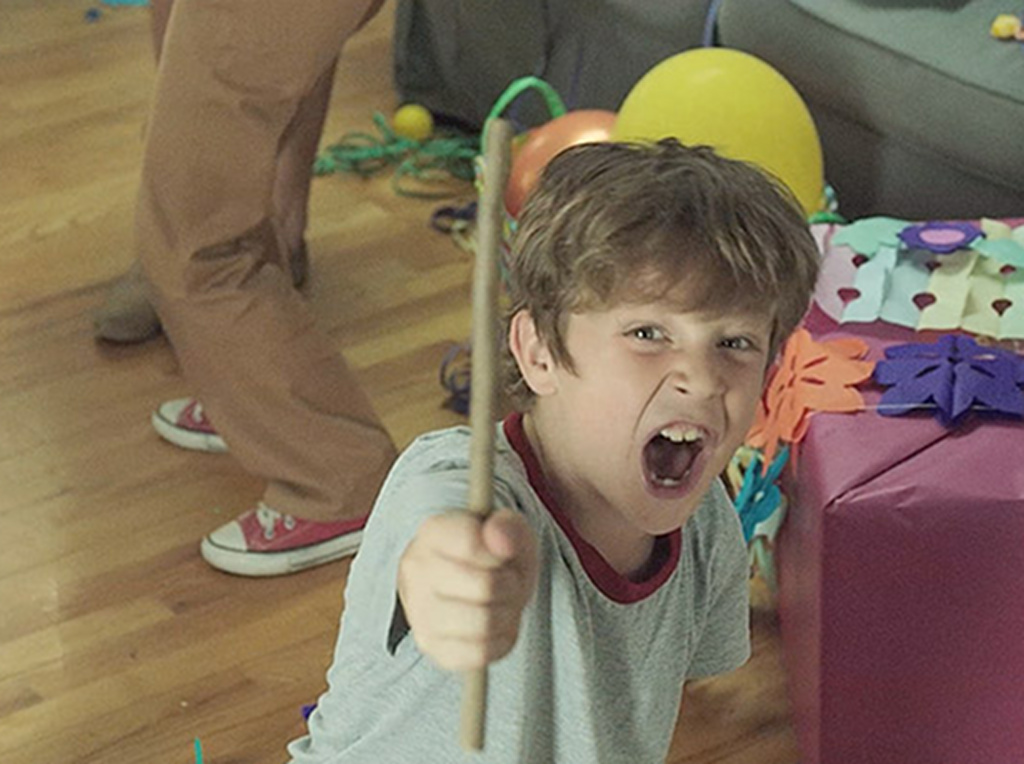
\includegraphics[height=1.0\paperheight]{pics/un-palo.jpg}}

\begin{frame}[plain]
  \vspace{6.25cm}
  \begin{TitleBox}
    {\LARGE \inserttitle} \\
    {\small Cuarenta características de Python que \textcolor{darkerred}{quizás} no conoces \\
     \insertauthor \enspace --- \thinspace \url{http://github.com/vterron}}
  \end{TitleBox}
\end{frame}
}
